%!TEX root = main.tex
% vim: tw=0 noet sts=8 sw=8



\section{Zusammenhang von Immersionen und Spinstrukturen}
\label{sec:Zusammenhang von Immersionen und Spinstrukturen}

Im folgenden ist $(M,g)$ eine geschlossene, orientierte Mannigfaltigkeit.
In der Notation wird die Metrik $g$ unterdrückt.


Um einen Zusammenhang zwischen den Immersionen und den Spinstrukturen
herzustellen ist es notwendig den Raum der Immersionen zu
vereinfachen.  Wichtig ist hierbei das wir nur an den
Zusammenhangskomponenten interessiert sind, also können wir uns nicht
nur auf Bijektionen sondern auch auf homotopieäquivalente Räume
einschränken.  Wir nennen zwei Immersionen $ \abb{f,g}{M}{N} $
\textit{regulär homotop} falls sie sich in $ \Imm{M}{N} $ durch einen
glatten Weg verbinden lassen.

Im Weiteren betrachten wir den Spezialfall $ M=M^2 $ Fläche und
$ N=\R^3 $.

Das Smale-Hirsch Theorem \cref{smalehirsch} liefert uns eine erste Vereinfachung des Raumes. 

Der Raum von formalen Immersionen lässt sich noch weiter verkleinern
bzw. vereinfachen, indem wir anstatt von nur formalen Immersionen auch
diese betrachten bei denen die Abbildungen zwischen den
Tangentialräumen auch noch isometrisch sind, damit erhalten wir
folgenden


\begin{Satz}\label{satz:immerformiso}
  Seien die isometrischen, formalen Immersionen gegeben durch
  \begin{gather*}
    \Immfi{M}{\R^3} \coloneqq \set{(f,F) \in \Immf{M}{\R^3}}{F \text{
        ist isometrisch }}.
  \end{gather*}
  Dann gilt das $\Immf{M}{\R^3}$ und $\Immfi{M}{\R^3}$
  homotopieäquivalent sind.
	\begin{proof}
          Betrachte für $t \in [0,1]$ die Abbildung
          $\abb{\psi_t}{\Immf{M}{\R^3}}{\Immf{M}{\R^3}}$ mit
          $\psi_t : (f,F) \mapsto (f,F \circ
          (F^{\ast}F)^{-t/2})$.
		
          Der Ausdruck $ (F_p^\ast F_p)^{-t/2} $ ist wie folgt
          definiert. Sei allgemein $ \abb{f}{V}{V} $ eine linearer, injektiver,
          symmetrischer Endomorphismus eines reellen Vektorraums mit
          Skalarprodukt gegeben. Da nun die Abbildung $ x\mapsto x^\alpha $ analytisch ist können wir die Potenzreihenentwicklung $ x^\alpha = \sum_{k=1}^{\infty} a_k x^k $ betrachten. Wir setzen dann $ f^\alpha \coloneqq \sum_{k=1}^{\infty} a_k f^k $. Die Konvergenz in $ V $ ist durch die Konvergenz der Potenzreihe garantiert.
		
          Des Weiteren ist diese Homotopie eine glatte Abbildung für alle
          $ t \in [0,1] $, wie man anhand der obigen Konstruktion erkennen kann. Für $ t=0 $ gilt $ \psi_0 = id $. Im Fall
          $ t=1 $ gilt nun das $ F \circ (F^{\ast}F)^{-t/2} $
          isometrisch ist.
		

%           dann existieren $ n $ positive, reelle
%          Eigenwerte $ \lambda_i $ für diesen Endomorphismus. Nach
%          Wahl einer Basis existiert eine unitäre Transformation
%          $ U $, sodass $ f = U^\ast \diag(\lambda_i) U $ gilt. Nun
%          definiere
%          $ f^\alpha \coloneqq U^\ast \diag(\lambda_i^\alpha) U $.
%          \todo{warum ist dies trotz der wahl wohldef?}
		
          Sei nun die lineare, injektive Abbildung
          $ \abb{F_p}{\tang{p}{M}}{\tang{F_p(p)}{\R^3}} $ gegeben,
          dann ist $ (F_p^\ast F_p) $ symmetrisch und aufgrund der
          Injektivität auch positiv definit, damit ist
          $ (F_p^\ast F_p)^{-1/2} $ wohldefiniert.
		
          Es folgt nun durch Umformungen das die Abbildung
          $ F_p \circ (F_p^\ast F_p)^{-1/2} $ isometrisch
          ist. Sei hierzu $ v,w \in \tang{p}{M} $,so gilt
          \begin{align*}
            \scalar{F_p \circ (F_p^\ast F_p)^{-1/2}(v)}{F_p \circ (F_p^\ast F_p)^{-1/2}(w)}_{\R^3} &=
                                                                                                                     g_p(F_p^\ast F_p \circ (F_p^\ast F_p)^{-1/2}(v),(F_p^\ast F_p)^{-1/2}(w)) \\
                                                                                                                   &= g_p((F_p^\ast F_p)^1/2(v),(F_p^\ast F_p)^{-1/2}(w)) \\
                                                                                                                   &= g_p((F_p^\ast F_p)^{-1/2} \circ (F_p^\ast F_p)^{1/2}(v,w)) \\
                                                                                                                   &= g_p(v,w)
		\end{align*}
		
		Hierbei haben wir $ \scalar{v}{F_p(w)}_{\R^3} = g_p(F_p^\ast(v),w) $ für $ q =F_p(p) $ und $ v \in \tang{q}{\R^3},w\in \tang{p}{M} $ 
		benutzt.
		
		Dann liefert dies die gewünschte Homotopieäquivalenz.
	
	\end{proof}
\end{Satz}

Der nächste Schritt ist der des Vergessens des Basispunktes.

\begin{Lem}\label{lem:famiso}
  Es existiert eine Bijektion
	
%	\begin{align*}
%		\Immfi{M}{\R^3} &\rightarrow \set{ (\abb{F_p}{\T_pM}{\R^3})_{p\in M} }{\text{ isometrisch}}\\
%	\end{align*}.
  \begin{tikzcd}
    \Immfi{M}{\R^3} \arrow[r,"\eta"] &%
    \set{ (\abb{F_p}{\TT_pM}{\R^3})_{p\in M} }{ F_p \text{ isometrisch, injektiv
        für alle }p \in M}.
  \end{tikzcd}
  \begin{proof}
    Definiere die Abbildung $ \eta $ wie folgt. Sei ein Paar
    $ (f,F) \in \Immfi{M}{\R^3}$ gegeben, dann setze als Zielobjekt
    die Familie $ (F_p)_{p\in M} $. Es ist noch zu zeigen
    das dies eine Bijektion ist.
    \begin{description}
    \item[Injektivität:] Seien zwei Paare $ (f,F),(g,G) $ mit
      $ \eta(f,F)=\eta(g,G) $ gegeben. Dann gilt nach Definition
      $ F_p = G_p $ für alle $ p\in M $. Also gilt $ F=G $ als
      Abbildungen. Da die Paare nun formale Immersionen sind gilt das
      die zugehörigen Diagramme aus \cref{formIso} kommutieren, also
      gilt:
      \begin{gather*}
        f \circ \pi^M = \pi_1 \circ F = \pi_1 \circ G = g \circ \pi^M
      \end{gather*}
      also
      \begin{gather*}
        f \circ \pi^M = g \circ \pi^M.
      \end{gather*}  Da die Projektion $ \pi^M $ surjektiv ist, folgt
      $ f=g $.  Also die Injektivität.
    \item[Surjektivität] Sei eine Familie $ (F_p)_{p\in M} $
      gegeben. Wähle eine beliebige glatte Funktion
      $ f\in \Cinfty{M}{\R^3} $. Setze nun als Urbild zu der anfangs
      gegebener Familie das Paar $ (f,F) $. Wobei $ F $ gegeben ist als
      \DefMap{\tang{}{M}}{\tang{}{\R^3}}{(p,v)}{(f(p),F_p(v)).}
			 
      Dann gilt offentsichtlich $ \eta(f,F)=(F_p)_{p\in M} $ und damit
      ist die Bijektivität nachgewiesen.
    \end{description}
  \end{proof}
\end{Lem}

Für das folgende Theorem benötigen wir die Existenz von Spinstrukturen
auf Flächen.
%lemma darüber das eine kompakte, orientierte 2dim riem mfg stets spin ist
\begin{Satz}\label{existenzspinflächen}
	Jede Fläche ist spin.
	\begin{proof}
		Wir haben schon in \cref{SpinstrSphäre} gezeigt das es 
		auf der $ \S^2 $ ein eindeutige Spinstruktur gibt. Wir
		wissen nun das sich alle Flächen als $ \S^2 $ mit Henkel 
		darstellen lassen.
		

		\begin{figure}[h]
		\begin{center}
			\includegraphics[width=5cm]{../pic/handles.png}
			\caption{Eine Fläche mit Geschlecht $ 3 $.}
		\end{center}
		\end{figure}
		
		 Um nun die Spinstruktur auf der $ \S^2 $
		auf Flächen mit höheren Geschlecht zu erweitern, müssen
		wir zeigen das ausgehend von der $ \S^2 $ und zwei Punkten
		$ p,q \in\S^2 $ mit disjunkten Bällen $ B_p,B_q \subset\S^2$,
		durch zusammenkleben der beiden Umgebungen ein Henkel
		entsteht und die Spinstruktur erhalten bleibt.
		
		Diese Chirugie gestaltet sich wie folgt. Wir wählen auf
		$ [0,1] \times \S^1 $ eine der beiden möglichen Spinstrukturen \footnote{hieran erkennt man schon das auf diese Art \textbf{nicht} alle $ 4 $ verschiedenen Spinstrukturen auf dem $ 2 $-Torus damit erhalten kann.} und betrachten 
		\begin{gather*}
		 \left. \left( \S^2 \setminus (B_p \cup B_q) \amalg [0,1]\times \S^1 \right) \right/_{\sim}  ~= \TT^2.
		\end{gather*}
		Wobei $ \partial B_p \sim \{ 0 \}\times \S^1$ und $ \partial B_q \sim \{ 1 \}\times \S^1$ miteinanderverklebt werden, sodass die Orientierung
		erhalten bleibt.
		Wir müssen nun zeigen das für zwei spin Mannigfaltigkeiten bei 
		der zusammenhängenden Summe ein eindeutige Spinstruktur existiert die 
		Erweiterungen der einzelnen Spinstrukturen ist.
	
		Hierzu betrachten wir zwei beliebige spin Mannigfaltigkeiten $ M,N $ und deren
		zusammenhängenden Summe $ M \# N $. Wir betrachten nun zu zwei Punkten
		$ p\in M,q\in N $ tubulare Umgebungen $ B_p,B_q $. Die Verklebung
		geschieht nun auf folgende Art. Wir verkleben den inneren Rand von $ B_p $
		mit	dem äußeren Rand von $ B_q $ und das gleiche mit $ p,q $ vertauscht.
		Wenn wir nun dieses Objekt einzeln betrachten und die induzierte Spinstruktur darauf lässt sich dieses Objekt als eine $ \S^n $ auffassen
		und mit \cref{Bsp:spinstrukturAufsphere} folgt nun das die darauf
		induzierte Spinstruktur eindeutig ist. Damit gibt es auf
		der zusammenhängenden Summe genau eine Erweiterung der
		einzelnen Spinstrukturen und mit der Methode des Henkels
		ankleben lässt sich auf jeder Fläche eine Spinstruktur finden.
	\end{proof}
\end{Satz}
% satz das die imm und form-imm homotop sind

Sei $\S M$ definiert als $\set{(p,v) \in \TT M}{ \norm{v} = 1}$, wobei
die Norm gegeben ist als $ \norm{(p,v)} \coloneqq \sqrt{g_p(v,v)} $
und wir der einfachheithalber lediglich $ \norm{v} $ schreiben werden.

Für den nächsten Satz benötigen wir miteinander verträgliche $ \S^1 $-Gruppenwirkungen auf der $ \S M $ und $ \so_3 $. Es wird die Identifizierung der Liegruppen $ \S^1 \simeq \so_2 $ vorausgesetzt. Für die erste
Gruppenwirkung wählen wir eine positiv orientierte Orthonormalbasis
$ (v,w) $ von $ \tang{p}{M} $ und betrachte den davon induzierten
Vektorraumisomorphismus $ \abb{\phi}{\R^2}{\tang{p}{M}},e_1 \mapsto v, e_2\mapsto w $. Diese
Abbildung liefert uns einen Liegruppenisomorphismus $\abb{\bar{\phi}}{\so(\R^2) = \so_2}{\so(\tang{p}{M})} $. Die Verkettung
dieser Isomorphismen liefert uns zu einem Element $ z\in\S^1 $ ein
eindeutiges Element $ U(z)\in \so(\tang{p}{M}) $. Damit ergibt sich
nun die Gruppenwirkung:
\DefMap{\S^1 \times \S_pM}{\S_pM}{(z,v)}{z*v\coloneqq U(z)v}

Für die zweite Gruppenwirkung benötigen wir den Fakt das sich jedes
Element $ A \in \so_3$  eindeutig in der Form $ A=\left( v~w~v\times w\right) $ mit $ v,w \in \R^3$ normiert und orthogonal zueinander, 
schreiben lässt. Durch die Wahl dieser Vektoren lässt sich auf
analoge Art wie oben ein Liegruppenisomorphismus $ \abb{\varphi}{\so_2}{\so(W)} $ finden, wobei $ W $ der von $ v,w $ 
im $ \R^3 $ aufgespannte Vektorraum ist. Damit operiert nun die
$ \S^1 $ auf dem $ \so_3 $.

Wir nennen nun eine glatte Abbildung $ \abb{H}{\S M}{\so_3}~\S^1$-invariant, falls $ H(z*v) = z*H(v) $ für alle $ z \in \S^1, v\in \S M $ gilt, also die Gruppenwirkung mit der Abbildung vertauscht. 
 

Der nächste Schritt wird der essentielle auf den Weg zu den
Zusammenhang mit den Spinstrukturen sein.

\begin{Satz}\label{satz:s1}
  Es existiert eine Bijektion zwischen
  \begin{gather*}
    \set{ (\abb{F_p}{\TT_pM}{\R^3})_{p\in M} }{ F_p \text{ isometrisch
        für alle }p \in M}
  \end{gather*}
  und
  \begin{gather*}
    \set{ \abb{H}{\S M}{\so_3}}{H\text{ ist }\S^1 \text{-invariant}}.
  \end{gather*}
  \begin{proof}
    Sei eine Familie $(\abb{F_p}{\TT_pM}{\R^3})_{p\in M}$ von
    isometrischen Abbildungen gegeben.  Da es sich bei $M$ um eine
    zweidimensionale, orientierte riemannische Mannigfaltigkeit
    handelt, gilt das zu es jedem normierten Tangentialvektor
    $v \in \S_p M$ genau einen Tangentialvektor $J(v) \in \S_p M$
    existiert, sodass $(v,J(v))$ eine positiv, orientierte
    Orthonormalbasis für $\tang{p}{M}$ bildet. Betrachte nun die
    Abbildung $\abb{H_p}{\S_p%
      M}{\so_3}, v \mapsto (F_p(v),F_p(J(v)),F_p(v)\times F_p(J(v)))$.
    Diese Abbildung ist wohldefiniert aufgrund der Eigenschaften der
    Basis $(v,J(v))$ und dass das Kreuzprodukt der beiden
    Basiselemente in Matrixform ein Element der $\so_3$ liefert, hier nutzen wir das die Abbildugen $ F_p $ isometrisch sind.  Die
    $\S^1$ Invarianz dieser Abbildung folgt direkt aus den oben
    konstruierten Gruppenwirkungen.   
	
    Zeige nun das es sich bei dieser Abbildung um eine Bijektion
    handelt.
    \begin{description}
    \item[Injektivität:] Seien zwei Familien $(F_p)_p,(G_p)_p$ von
      isometrischen Abbildungen gegeben und sei
      $\vartheta((F_p)_p)=\vartheta((G_p)_p)$. Dann gilt aufgrund der
      Abbildungsvorschrift von $\vartheta$ das $F_p(v)=G_p(v)$ für
      alle $v \in \S_p M$ gilt und somit die Abbildungen gleich sind.
    \item[Surjektivität:] Sei eine $\S^1$-invariante Abbildung
      $\abb{H}{\S M}{\so_3}$ gegeben. Für einen normierten
      Tangentialvektor $v \in \S_p M$ gilt das $H_p(v)$ ein Element
      der $\so_3$ ist. Betrachte nun die erste Spalte der Matrix
      $w(v)=(H_p(v)_{i,1})_{i=1,2,3}$. Definiere nun eine Abbildung
      $\abb{F_p}{\tang{p}{M}}{\R^3}$ durch $v \mapsto \begin{cases}
        w(\frac{v}{\norm{v}}) & v \neq 0 \\
        0 & v=0.
      \end{cases}$
		
      Diese Abbildung liefert uns nun das gewünschte Urbild zur
      anfangs gewählten Abbildung $H$.
    \end{description}
    Der Nachweis der Bijektion liefert die Behauptung.
\end{proof}

\end{Satz}

Für den schlussendlichen Satz dieser Arbeit benötigen wir noch einige
Homotopiegruppen der $\so_3$ und $\spin_3$. Die verwendete Quelle ist
hierbei \cite{BHMMM15}.
\begin{Lem}\label{hgroups}
	Für die beiden Liegruppen $\spin_3$ und $\so_3$ gelten
	folgende Isomorphien als Mannigfaltigkeiten:
	\begin{align}
	\spin_3 &\simeq \su(2) \simeq \S^3 \label{id1}\\
	\so_3 &\simeq \RP^3 \label{id2}
	\end{align}
	Damit gelten auch folgende Isomorphien der Homotopiegruppen
	der beide Liegruppen.
	\begin{align*}
	\pi_k(\spin_3) &\simeq \begin{cases}
	1 & ,k=0,1,2 \\
	\Z & ,k=3
	\end{cases}
	&{\pi_k(\so_3) \simeq \begin{cases}
		1 & ,k=0,2 \\
		\Z_2 & ,k=1 \\
		\Z & ,k=3
		\end{cases}}
	\end{align*}
	
	\begin{proof}
		\begin{description}
                \item[1. Schritt:] Wir wollen zunächst die zweite
                  Identität \cref{id1} zeigen. Dieser Isomorphismus
                  ist direkt durch folgende Abbildung anzugeben
                  \DefMap{\set{\pma{a & -\bar{b} \\ b & \bar{a}} \in
                      \su_2}{a,b \in \c}}{\set{(a,b)\in
                      \c^2}{|a|^2+|b|^2=1}=\S^3}{\pma{a & -\bar{b} \\
                      b & \bar{a}}}{(a,b)}
			
                  Von \cref{id1} die erste Identität wird wie folgt
                  bewiesen.  Es gilt zunächst das die Spingruppe
                  $ \spin_3 $ eine Teilmenge der Cliffordalgebra
                  $ \Cl_3 $ ist und im geraden Teil dieser liegt, also
                  eine Untergruppe von $ \H^\ast $ ist. Man kann nun
                  zeigen das dies schon die gewünschte Behauptung
                  zeigt das $ \spin_3 \simeq \su_2 $ gilt.
				  Es folgt nun unmittelbar aufgrund des Isomorphismus
				  und den doppelten Überlagerung durch rausteilen
				  von $ \Z_2 $ die Isomorphie $ \RP^3\simeq\so_3 $.
			
                \item[2. Schritt;] Seien nun die obigen Identitäten
                  \cref{id1} gegeben, um nun die
                  die Homotopiegruppen zu berechnen reicht es aus
                  diese von $\RP^3$ und $ \S^3 $ zu kennen. Für
                  $ \S^3 $ sind diese bekannt und für $ \RP^3 $
                  stimmen diese für $ k \neq 1 $ mit denen von
                  $ \S^3 $ überein. Die Fundamentalgruppe von
                  $ \RP^3 $ ist bekannterweise $ \Z_2 $. Somit ist
                  alles gezeigt.
		\end{description}
		
		
		
	\end{proof}
	
\end{Lem}

Nach dieser weiteren Vereinfachung des Raums der Immersionen folgt nun
der letzte Schritt. Wir können nun folgenden Satz zeigen.



\begin{Satz}\label{satz:spinstrukturen}
	Es existiert eine Bijektion
	\begin{center}
		\begin{tikzcd}
			\set{ \abb{H}{\S M}{\so_3}}{H\text{ ist }\S^1 \text{-invariant}}/\sim  \arrow[rr,"\psi"] && \sset{\text{Spinstrukturen auf }M}/\sim.\\
		\end{tikzcd}
	\end{center}
	Wobei $ \sim $ links bis auf Homotopie und rechts bis auf Isomorphie meint.
	\begin{proof}

%          Wir können zu auf folgende Art und Weise eine Abbildung
%          $\psi$ konstruieren.  Zu einer $\S^1$-invarianten Abbildung
%          $\abb{H}{\S M}{\so_3}$ definieren wir zunächst eine
%          Spinstruktur auf dem $0$-Skelett und setzen diese induktiv
%          auf die höheren Skelette fort um schließlich beim
%          $2$-Skelett endend auf der gesamten Mannigfaltigkeit eine
%          Spinstruktur zu erhalten. Schließlich zeigen wir noch das
%          diese Konstruktion eine Bijektion liefert.
		Wir wollen zunächst die Abbildung angeben.
		
          \textbf{Konstruktion der Abbildung $\psi$}
		
          Sei eine $\S^1$-invariante Abbildung
          $\abb{H}{\S M}{\so_3}$ gegeben. Die Spinstruktur zu $ H $
          sei nun gegeben durch den Pullback entlang der Abbildung $ H $
          gegeben.
              \begin{center}
              \begin{tikzcd}
                H^\ast\Ad  =\Ph{\spin_2}{M} \arrow[r,"\phi"] \arrow[d] \arrow[dr, phantom, "\ulcorner", very near start] & \spin_3 \arrow[d,"\Ad"] \\
                \Ph{\so_2}{M} = \S M \arrow[r,"H"] & \so_3
              \end{tikzcd}
            \end{center}
          Die so erhaltende Mannigfaltigkeit $ \Ph{\spin_2}{M} $ ist ein
          $ \spin_2 $-Hauptfaserbündel. Die $ \spin_2 $-Gruppenwirkung
          ist durch
          \DefMap{\spin_2 \times \Ph{\spin_2}{M}}{\Ph{\spin_2}{M}}{(z,p)}{z\phi(p)}
          gegeben. Wobei wir die kanonische Identifzierung $ \spin_2\subset\spin_3 $ benutzt haben. Die Gruppenwirkung ist
          glatt aufgrund der universellen Eigenschaft des Pullbacks.
%          Spinstruktur
%          auf $ M $. Diese ist eine zweifache Überlagerung des orientieren
%          Rahmenbündels und hat eine $ \spin_2 $-Gruppenwirkung durch
%          eine Wahl $ \spin_2\subset\spin_3 $ und den Morphismus $ \phi $.
	       Im nächsten Schritt müssen wir zeigen das diese Konstruktion
	        homotopieinvariant ist, d.h. für homotope Abbildungen $ H,H^{'} $ die induzierten Spinstrukturen isomorph sind.
	        
          Hierzu wählen wir eine Triangulierung $\Sigma \coloneqq \sset{ \Delta_i^j}$ der Mannigfaltigkeit, um den Beweis der Bijektivität entlang des Skeletts zu führen. Wobei für den Simplex $\Delta_i^j$ der
          Index $i$ einer Durchnummerierung entspricht und der Index
          $j$ die Dimension des Simplex angibt. 
          \begin{center}
          	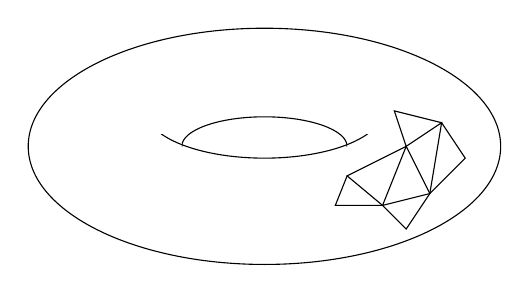
\begin{tikzpicture}[scale=1.5]
          	\draw ellipse (2cm and 1cm);
          	\begin{scope}
          	\clip (-0.7,0)rectangle(0.7,0.5);
          	\draw ellipse (0.7cm and 0.25cm);
          	\end{scope}
          	\begin{scope}
          	\clip (-0.9,0.1)rectangle(0.9,-0.5);
          	\draw (0,0.3) ellipse (1cm and 0.4cm);
          	\end{scope}
          	%              	\draw [thin] (0,0) to (1,0) to (0,1) to (0,0);
          	\draw [thin] (1,-0.5) to (1.2,0) to (1.4,-0.4) to (1,-0.5);
          	\draw [thin] (1.2,0) to (1.5,0.2) to (1.4,-0.4); 
          	\draw [thin] (1,-0.5) to (0.7,-0.25)  to (1.2,0) ;
          	\draw [thin] (1,-0.5) to (1.2,-0.7) to (1.4,-0.4)  ; 
          	\draw[thin] (1.5,0.2) to (1.7,-0.1) to (1.4,-0.4); 
          	\draw [thin] (1.2,0) to (1.1,0.3) to (1.5,0.2);
          	\draw [thin] (1,-0.5) to (0.6,-0.5) to (0.7,-0.25) ;
          	\end{tikzpicture}
          \end{center}
	        \todo{mehr simplizies einführen}
	       Wir zeigen nun die Bijektivität von $ \psi $.
          
          \begin{description}
	          	\item[Injektivität:] Seien $ \abb{H,H^{'}}{\S M}{\so_3} $
	          	zwei $ \S^1 $-invariante Abbildungen mit $ \psi(H)=\psi(H^{'}) $. Wir wollen zeigen das die beiden
	          	Abbildungen homotop zueinander sind. Hierzu nutzen wir
	          	die Skelettstruktur der Mannigfaltigkeit aus.
		          	\begin{enumerate}[1{\bfseries -Skelett:}]
		          		\item[$ 0 ${\bfseries-Skelett:}] Für die endlich vielen $ 0 $-Skelette, also
		          		Punkte, auf der Mannigfaltigkeit lässt sich durch
		          		eine beliebige Verschiebung die Gleichheit von
		          		den Werten der beiden Abbildungen $ H,H^{'} $
		          		erreichen.
		          		\item Seien die Abbildungen auf dem $ 0 $-Skelett
		          		gleich, dann betrachten wir eine Kurve $ \gamma $
		          		die genau einen $ 1 $-Simplex durchläuft.
		          		Die Abbildung $ \abb{\dfrac{\dot{\gamma}}{\norm{\dot{\gamma}}}}{\S^1}{\S M = \Ph{\so}{M}} $ liftet genau dann auf $ \Ph{\spin}{M} $ wenn die Abbildungen
		          		$ H,H^{'} \circ \dfrac{\dot{\gamma}}{\norm{\dot{\gamma}}} $ auf
		          		$ \spin_3 $ liften. Das heißt das 
		          		\begin{gather*}
		          			 \left[H^{'} \circ \dfrac{\dot{\gamma}}{\norm{\dot{\gamma}}} \right]
		          			 = \left[ H \circ \dfrac{\dot{\gamma}}{\norm{\dot{\gamma}}} \right] \in \pi_1(\so_3)=\Z_2
		          		\end{gather*}
		          		Falls die Elemente in verschiedenen Klassen 
		          		liegen, ändere eine der beiden Klassen wie folgt
		          		ab. Sei $ [\eta] $ ein Erzeuger von $ \pi_1(\so_3) $ und durchlaufe diesen zuerst
		          		und dann jeweils die entsprechende Klasse, dann
		          		stimmen die beiden Klassen in der Fundamentalgruppe überein.
		          		
		          		
			          	\item \OE~Seien die Abbildungen auf dem $ 1 $-Skelett gleich, dann betrachten wir die
			          	Einschränkungen der $ H_i $ auf $ \S \Delta^2 = D^2 \times \S^1$. Wir erhalten ein Diagramm
			          	von der Form
			          	
			          	\begin{center}
			          		\begin{tikzcd}
			          			\S \Delta^2 \arrow[r,"H_i"] & \so_3 \\
			          			D^2 \arrow[u, "\iota"] \arrow[ur, "\hat{H}_i"'] 
			          		\end{tikzcd}
			          	\end{center}
			          	
			          	Wir nutzen nun ein allgemeines Lemma.
			          	
			          	\begin{Lem}
		          		Sei $ n\geq 2 $ und $ X $ ein topologischer Raum mit
		          		$ \pi_n(X)=0 $ und 
		          		$ \abb{f,g}{D^n}{X} $ zwei stetige Abbildungen
		          		für die $ f_{|\S^{n-1}} = g_{|\S^{n-1}} $ gilt, dann
		          		sind $ f,g $ homotop.
			          	\end{Lem}
			          	
			          	Da die Abbildungen nach Voraussetzung auf 
			          	dem Rand des Simplex $ \Delta^2 $ übereinstimmen
			          	und $ \pi_2(\so_3)=0 $ nach \cref{hgroups} gilt sind die beiden
			          	Abbildungen homotop auf $ \Delta^2 $. Dies setzt
			          	sich nun auf $ \S \Delta^2 $ fort. Damit sind
			          	die Abbildungen auf dem $ 2 $-Skelett homotop, 
			          	also auch auf der Mannigfaltigkeit selbst.
		          	\end{enumerate}
		  \item[Surjektivität:] Sei nun eine Spinstruktur $ \Ph{\spin_2}{M} $ auf $ M $
		  vorgegeben. Wir müssen eine $ \S^1 $-invariante Abbildung
		  konstruieren die diese Spinstruktur induziert.
		  
		  Wir benutzen hierzu die Triangulierung und damit die Zerlegung
		  der Mannigfaltigkeit $ M $ in Skelette $ M_0\subset M_1\subset M_2 $.
		  Wir werden nun über das Skelett ein Urbild zu der Spinstruktur
		  konstruieren.
%		  
		  \begin{enumerate}[1{\bfseries -Skelett:}]
		  	\item[$ 0 ${\bfseries-Skelett:}] Es gilt für das $ 0 $-Skelett
		  	und die Strukturen:
			  	\begin{gather*}
			  		\Ph{\spin_2}{M_i} \coloneqq \pi^{-1}_{\spin}(M_i)\\
			  		\Ph{\so_2}{M_i} \coloneqq \pi^{-1}_{\so}(M_i)
			  	\end{gather*}
			  	Nun lässt sich eine $ \S^1 $-invariante Abbildung
			  auf $ \Ph{\so_2}{M_0} $ angeben durch eine beliebige Wahl
			  von Elementen aus von einem $ v\in \S M_0 $ und 
			  $ \so_3 $ und mit der Forderung der $ \S^1 $-Invarianz
			  ist die Abbildung wohldefiniert. Diese Abbildung
			  liftet nun auf eindeutige Art zu einer Abbildung auf
			  $ \Ph{\spin_2}{M_0} \to \spin_3$. Damit ist $ H $ auf dem
			  $ 0 $-Skelett vorgegeben.
		  	\item Wir betrachten nun einen Weg in $\abb{\gamma}{[0,1]}{\Ph{\spin_2}{M_1}} $ der entlang eines $ 1 $-Simplex
		  		verläuft und am $ 0 $-Skelett dessen mit der obigen Abbildung $ H $
		  		übereinstimmt. Da nun $ \pi_0(\spin_3)=0 $ gilt, können wir
		  		diesen Weg zu $ \bar{\gamma} \colon [0,1] \to \Ph{\spin_2}{M_1} \to \spin_3 $ fortsetzen. Wir können nun diese Abbildung runterdrücken
		  		durch die jeweiligen doppelten Überlagerungen und damit die
		  		Abbildung $ H $ auf das $ 1 $-Skelett fortsetzen. Die $ \S^1 $-Invarianz der Abbildung bleibt aufgrund der verschwindenden
		  		$ \pi_1(\spin_3)=0 $ gewahrt.
		  	\item Sei nun die zu konstruierende Abbildung $ H $ auf dem $ 1 $-Skelett
		  	vorgegeben. Um diese auf das $ 2 $-Skelett fortzusetzen betrachten
		  	wir die Abbildung $ \abb{H}{\Ph{\spin_2}{M_1}}{\spin_3} $ auf
		  	den Rand eines einzelnen $ 2 $-Simplex $ \Delta $. Um die Abbildung auf das Innere
		  	dieses $ 2 $-Simplex eindeutig fortzusetzen benötigen wir den 
		  	allgemeinen 
		  	\begin{Satz}
		  	Falls $ (W,A) $ ein zusammenhängender, abelscher $ CW $ Komplex ist und  ein Diagramm der Art
		  	\begin{center}
		  		\begin{tikzcd}
		  			A \arrow[d, hook] \arrow[r] & X \\
		  			W \arrow[ru, dashed]
		  		\end{tikzcd}
		  	\end{center}
		  	gegeben, dann existiert der getrichelte Pfeil falls $ H^{n+1}(W,A,\pi_n(X)) =0$ erfüllt ist.
		  	\end{Satz}
		  	Falls man nun $ A=\Ph{\spin_2}{\partial\Delta} ,W=\Ph{\spin_2}{\Delta} $ und $ X=\spin_3 $ setzt, gilt mit $ \pi_2(\spin_3)=0 $ die hinreichende
		  	Bedingung des obigen Satzes und damit lässt sich die Abbildung bis
		  	auf Homotopie auf das $ 2 $-Skelett fortsetzen. Um nun eine $\S^1$ Abbildung
		  	$\Ph{\so_2}{M_2} \to \so_3$ zu bekommen geht man vor wie in dem Schritt 
		  	beim $ 1 $-Skelett.
		  \end{enumerate}
		  Nun ist die Abbildung $ H $ auf der Mannigfaltigkeit konstruiert die
		  die Spinstruktur induziert.
          \end{description}
          Damit ist die Behauptung des Satzes gezeigt.
	\end{proof}
\end{Satz}

Schlussendlich lässt sich das Hauptresultat dieser Arbeit in einem Theorem
formulieren.

\begin{Thm}
	Sei $ (M,g) $ eine Fläche, dann gilt 
	\begin{gather*}
	 \pi_0(\Imm{M}{\R^3}) = \sset{\text{Spinstrukturen auf }M}/\sim  
	\end{gather*}
	Das heißt die Zusammenhangskomponenten
	des Raums aller Immersionen stehen in Bijektion zu den Spinstrukturen der Fläche.
	\begin{proof}
		In diesem Beweis werden lediglich die vorherigen bewiesenen Sätze benutzt
		um das Resultat zu zeigen.
		Ausgehend von \cref{smalehirsch} können wir uns auf die formalen Immerisonen
		einschränken, die durch \cref{satz:immerformiso} homotopieäquivalent zu
		den formalen isometrischen Immserionen sind. Weiter können wir durch
		\cref{lem:famiso} uns auf Familien von isometrischen, injektiven Abbildungen
		in den $ \R^3 $ einschränken. Nun wird durch \cref{satz:s1} eine Bijektion
		zu $ \S^1 $-invarianten Abbildungen hergestellt und damit schließlich 
		eine Bijektion in \cref{satz:spinstrukturen} zu den Spinstrukturen.
		In all diesen Sätzen und Lemmata sind die Zusammenhänge Bijektionen oder
		Homotopieäquivalenzen. Der Funktor $ \pi_0 $ ist invariant unter diesen
		Isomorphismen und liefert damit die gewünschte Behauptung.
	\end{proof}
\end{Thm}



%% Local Variables:
%% mode: latex
%% TeX-master: "main"
%% End:
